\documentclass[letterpaper,11pt]{article}

\usepackage{amsmath,amssymb,amsthm}
\usepackage[margin=2.0cm]{geometry}
\usepackage{float}
\usepackage{tikz}

\usetikzlibrary{arrows,automata}

\newcommand{\N}{\mathbb{N}}

\newtheorem{proposition}{Proposition}

\title{Assignment \#1}
\author{Jacob Thomas Errington}
\date{24 September 2015}

\begin{document}

\maketitle

\begin{description}
    \item[Question \#1] A finite alphabet $\Sigma$ is fixed.

        \begin{enumerate}
            \item Let $x,y\in\Sigma^*$. If $x$ is a prefix of $y$, then
                $\exists z_1 \in\Sigma^* \, y = xz_1$ and if $y$ is a prefix of
                $x$, then $\exists z_2\in\Sigma^* \, x = y z_2$.

                \begin{proposition}
                    If $x$ and $y$ are prefixes of each other, then $x = y$.
                \end{proposition}

                \begin{proof}
                    By contradiction.

                    Assume $z_1 z_2 \neq \epsilon$.

                    \begin{align}
                        x &= y z_2 \notag \\
                        x &= (xz_1) z_2 \notag \\
                        x &= x z_1 z_2
                        \label{eq:prefix_eachother}
                    \end{align}

                    This is a contradiction. Thus, $z_1 z_2$ must be empty. In
                    turn, the concatenation of two strings is the empty string
                    only if the two strings being concatenated are themselves
                    the empty string as well. (In monoids, there is no notion
                    of inverses, unlike in groups.)

                    Hence, $x = y z_2 = y$.
                \end{proof}

            \item Let $\Sigma = \{a,b\}$. Let $\#_a(x)$
                denote the number of occurrences of the letter
                $a$ in $x$.

                \begin{proposition}
                    $$
                    \forall x\in\Sigma^*\,
                    \exists y,z\in\Sigma^*:
                    x=yz\land[\#_a(y)=\#_b(z)]
                    $$

                    For any word, we can cut it into two parts such that the
                    number of occurences of $a$ in the first part is equal to
                    the number of occurences of $b$ in the second part.
                \end{proposition}

                \begin{proof}
                    By induction.

                    For the empty string, there is only a trivial cut, and the
                    two resulting parts are also the empty string. Naturally,
                    the number of occurences of $a$ in the first part matches
                    the number of occurences of $b$ in the second.

                    Inductive hypothesis: $x = yz$ such that
                    $\#_a(y) = \#_b(z)$.

                    We seek to append one character to $x$ to form
                    $x^\prime=y^\prime z^\prime$. We will analyze both
                    possibilities of characters to add.

                    If $x^\prime=xa$,
                    then let$y^\prime=y$
                    and
                    $z^\prime=za$.
                    We observe $\#_a(y^\prime)=\#_a(y)$
                    and
                    $\#_b(z^\prime)=\#_b(z)$.
                    Thus, this new proposed cut satisfies the proposition.

                    If $x^\prime=xb$, then
                    let $z_1\in\Sigma\,z_1w=z$,
                    $y^\prime=yz_1$
                    and
                    $z^\prime=wb$.

                    If $z_1=a$,
                    then $\#_a(y^\prime)=\#_a(y)+1$
                    and
                    $\#_b(z^\prime)=\#_b(z)+1$,
                    so
                    $\#_a(y^\prime)=\#_b(z^\prime)$.

                    If $z_1=b$,
                    then $\#_a(y^\prime)=\#_a(y)$
                    and
                    $\#_b(z^\prime)=\#_b(z)$,
                    so
                    $\#_b(y^\prime)=\#_b(z^\prime)$.
                    Thus, this new proposed cut satisfies the proposition.

                    Since we can find a valid cut in the trivial case of the
                    empty string, and since we can find a valid cut for a
                    string built by appending one more character, weareable,
                    by induction, to find valid cuts for strings of arbitrary
                    length.
                \end{proof}
        \end{enumerate}

\item[Question \#2] A finite alphabet $\Sigma$ is fixed, and let
    $\emptyset \neq L\subseteq\Sigma^*$. Consider the following relation.

    $$
    \forall x,y\in\Sigma^* : xRy
    \text{if}
    \forall z \in \Sigma^* :
        xz \in L
        \iff
        yz \in L
    $$

    \begin{proposition}
        $R$ is an equivalence relation.
    \end{proposition}

    \begin{proof}
        We will verify the requirements for being an equivalence relation.

        \begin{description}
            \item[Reflexivity.]
                It is trivially true that $xRx$ since $p \iff p$ is true
                forall $p$.

            \item[Symmetry.]
                Assume $xRy$, i.e.
                $\forall z \in \Sigma^* : xz \in L \iff yz \in L$.
                The if-and-only-if logical connective is symmetric, so we
                have
                $\forall z \in \Sigma^* : yz \in L \iff xz \in L$.
                This is precisely the requirement for $yRz$.

            \item[Transitivity.]
                Assume $wRx$ and $xRy$, i.e.
                \begin{align*}
                    \forall z:
                    (wz\in L\iff xz\in L)
                    \land
                    (xz\in L\iff yz\in L)
                \end{align*}

                The truth values of
                $wz \in L$ and $yz \in L$
                are both equivalent to the truth value of
                $xz \in L$.
                Hence,
                $wz \in L \iff yz \in L$.
                In other words, the transitivity of $R$ follows from the
                transitivity of $\iff$.
        \end{description}

        Since $R$ satisfies the above three criteria, it is an equivalence
        relation.
    \end{proof}

\item[Question \#3]
    Consider $\N\times\N$ with the binary lexicographic ordering relation
    $\sqsubseteq$ defined by the following.

    $$
    (m,n)\sqsubseteq(m^\prime,n^\prime)
    \iff
    m<m^\prime
    \lor
    (m=m^\prime\land n\leq n^\prime)
    $$

    \begin{proposition}
        The binary lexicographic ordering relation is a partial order on
        $\N\times\N$.
    \end{proposition}

    \begin{proof}
        We will verify the three conditions on being a partial order.

        \begin{description}
            \item[Reflexivity.]
                Let $m^\prime=m$ and $n^\prime=n$ in the definition of
                the lexicographic ordering relation. The following
                statement is the result of that substitution.

                $$
                m<m\lor(m=m\land n\leq n)
                $$

                This statement is true, and is precisely the requirement
                for being reflexive.

            \item[Anti-symmetry.]
                Assume the following two propositions.

                \begin{align}
                    (m,n)&\sqsubseteq(m^\prime,n^\prime)\label{eq:as1}\\
                    (m^\prime,n^\prime)&\sqsubseteq(m,n)\label{eq:as2}
                \end{align}

                Assume $m<m^\prime$. This can not be the case, as it would
                contradict a result we obtain from
                \eqref{eq:as2}, namely that
                $m^\prime<m\lor m^\prime=m\land n^\prime\leq n$.
                A symmetrical argument shows that it can neither be the
                case that $m^\prime<m$.
                Hence,
                $m = m^\prime \land n \leq n^\prime$.
                Likewise,
                $m^\prime = m \land n^\prime \leq n$.
                Thus,
                $n = n^\prime$,
                and we conclude finally that given our initial two
                assumptions,
                $(m, n) = (m^\prime, n^\prime)$.

            \item[Transitivity.]
                Assume the following two propositions.

                \begin{align*}
                    (m_1,n_1)&\sqsubseteq(m_2,n_2)\\
                    (m_2,n_2)&\sqsubseteq(m_3,n_3)
                \end{align*}

                In particular, we have the following.

                \begin{align}
                    m_1<m_2 &\lor m_1 = m_2 \land n_1 \leq n_2
                        \label{eq:trans1} \\
                    m_2<m_3 &\lor m_2 = m_3 \land n_2 \leq n_3
                        \label{eq:trans2}
                \end{align}

                If $m_1 < m_2 \lor m_2 < m_3$, then $m_1 < m_3$.
                Hence, $(m_1, n_1) \sqsubseteq (m_3, n_3)$.

                If $m_1 = m_2 = m_3$, then $n_1 \leq n_2 \leq n_3$, which
                implies $n_1 \leq n_3$.
                Hence, $(m_1, n_1) \sqsubseteq (m_3, n_3)$.

                This covers all the possible cases that can result from our
                initial two assumptions. Thus, transitivity holds.
        \end{description}

        Thus, $\sqsubseteq$ is a partial order on $\N \times \N$.
    \end{proof}

    \begin{proposition}
        The binary lexicographic ordering on $\N \times \N$ is a well-founded
        order.
    \end{proposition}

    \begin{proof}
        Consider $S \neq \emptyset \subseteq \N \times \N$.

        Select
        $$
        S_1 = \{
            (m, n) \in S
            | \forall (m^\prime, n^\prime) \in S : m \geq m^\prime
        \}
        $$

        In other words, select $S_1$ such that its elements have minimal
        \emph{first} components within $S$.

        Then, select
        $$
        S_2 = \{
            (m, n) \in S_1
            | \forall (m^\prime, n^\prime) \in S_1 : n \geq n^\prime
        \}
        $$

        In other words, select $S_2$ such that its elements have minimal
        \emph{second} components within $S_1$. Note that both $S_1$ and $S_2$
        are nonempty due to the well-ordering principle on naturals.

        Now, assume for some
        $(m, n) \in S_2$
        there exists
        $(m^\prime, n^\prime) \in S$
        such that
        $(m^\prime, n^\prime) \sqsubseteq (m, n)$.
        This would mean
        $m^\prime < m \lor m^\prime = m \land n^\prime \leq n$.

        Recall that $m$ is such that it is minimal as a first component of
        elements of $S$.
        Hence, it cannot be the case that $m^\prime < m$;
        it must be that
        $m^\prime = m$,
        and thus that
        $(m^\prime, n^\prime) \in S_1$.

        However, recall that $n$ is such that it is minimal as a second
        component of elements of $S_1$.
        Hence, it cannot be the case that $n^\prime < n$;
        it must be that
        $n^\prime = n$,
        and thus that
        $(m^\prime, n^\prime) = (m, n)$.

        In conclusion, any nonempty subset of $\N \times \N$ has a minimal
        element, which we can construct from the above two-stage selection
        process.
    \end{proof}

\item[Question \#4]
    The following DFAs recognize languages on the alphabet $\{0,1\}$.

    \begin{enumerate}
        \item The DFA in figure \ref{fig:dfa:00} recognizes strings ending with
            two zeros.

            \begin{figure}[H]
                \centering

                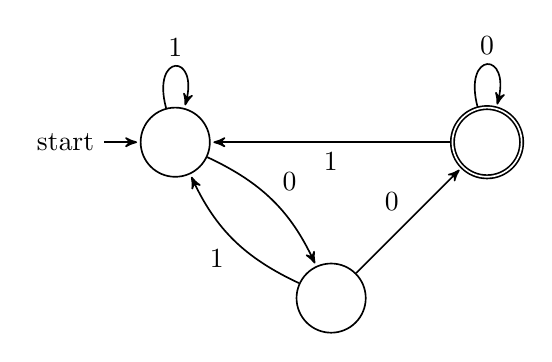
\begin{tikzpicture}[
                        ->,
                        >=stealth',
                        shorten >=1pt,
                        auto,
                        node distance=2.8cm,
                        semithick
                    ]
                    \tikzstyle{every state}=[fill=white,draw=black,text=black]

                    \node[initial,state]   (A) {} ;
                    \node[state]           (B) [below right of=A] {} ;
                    \node[accepting,state] (C) [above right of=B] {} ;

                    \path
                    (A) edge [loop above]   node {1} (A)
                    (A) edge [bend left=20] node {0} (B)
                    (B) edge [bend left=20] node {1} (A)
                    (B) edge                node {0} (C)
                    (C) edge                node {1} (A)
                    (C) edge [loop above]   node {0} (C) ;
                \end{tikzpicture}
                \label{fig:dfa:00}

                \caption{A DFA to recognize strings ending with two zeroes.}
            \end{figure}

        \item The DFA in figure \ref{fig:dfa:2zero2one} recognizes strings
            ending with either two zeros or two ones.

            \begin{figure}[H]
                \centering

                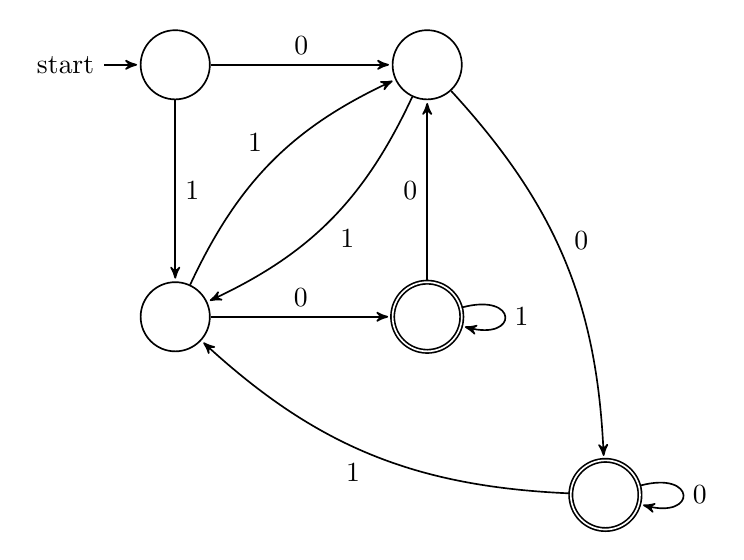
\begin{tikzpicture}[
                        ->,
                        >=stealth',
                        shorten >=1pt,
                        auto,
                        node distance=3.2cm,
                        semithick
                    ]
                    \tikzstyle{every state}=[fill=white,draw=black,text=black]

                    \node[initial,state]   (A)                    {} ;
                    \node[state]           (B) [right of=A]       {} ;
                    \node[state,accepting] (D) [below of=B]       {} ;
                    \node[state,accepting] (C) [below right of=D] {} ;
                    \node[state]           (E) [below of=A]       {} ;

                    \path
                    (A) edge                node {0} (B)
                    (A) edge                node {1} (E)
                    (B) edge [bend left=20] node {0} (C)
                    (B) edge [bend left=20] node {1} (E)
                    (C) edge [loop right]   node {0} (C)
                    (C) edge [bend left=20] node {1} (E)
                    (D) edge                node {0} (B)
                    (D) edge [loop right]   node {1} (D)
                    (E) edge                node {0} (D)
                    (E) edge [bend left=20] node {1} (B) ;

                \end{tikzpicture}
                \label{fig:dfa:2zero2one}

                \caption{A DFA to recognize strings ending with either two
                zeros or two ones.}
            \end{figure}

        \item The DFA in figure \ref{fig:dfa:secondlast1} recognizes strings
            whose second last character is a $1$.

            \begin{figure}[H]
                \centering

                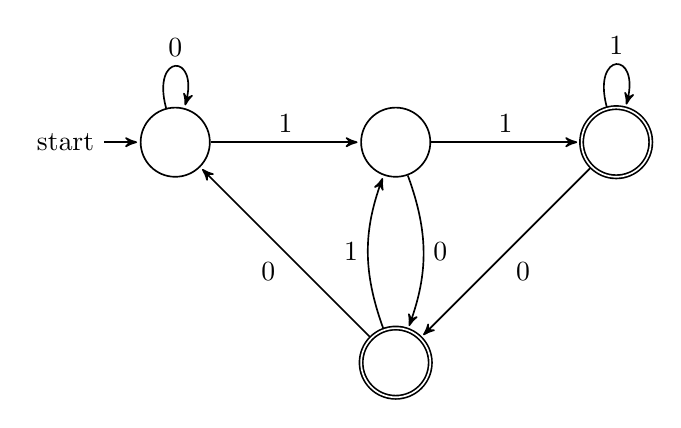
\begin{tikzpicture}[
                        ->,
                        >=stealth',
                        shorten >=1pt,
                        auto,
                        node distance=2.8cm,
                        semithick
                    ]
                    \tikzstyle{every state}=[fill=white,draw=black,text=black]

                    \node[initial,state]   (A)                    {} ;
                    \node[state]           (B) [right of=A]       {} ;
                    \node[state,accepting] (C) [right of=B]       {} ;
                    \node[state,accepting] (D) [below of=B] {} ;

                    \path
                    (A) edge [loop above]   node {0} (A)
                    (A) edge                node {1} (B)
                    (B) edge [bend left=20] node {0} (D)
                    (B) edge                node {1} (C)
                    (C) edge                node {0} (D)
                    (C) edge [loop above]   node {1} (C)
                    (D) edge                node {0} (A)
                    (D) edge [bend left=20] node {1} (B) ;

                \end{tikzpicture}
                \label{fig:dfa:secondlast1}

                \caption{A DFA to recognize strings whose second last character
                is $1$.}
            \end{figure}
    \end{enumerate}

\item[Question \#5]
    \begin{enumerate}
        \item The DFA in figure \ref{fig:dfa:contain100110} recognizes strings
            containing the substrings $100$ or $110$.

            \begin{figure}[H]
                \centering

                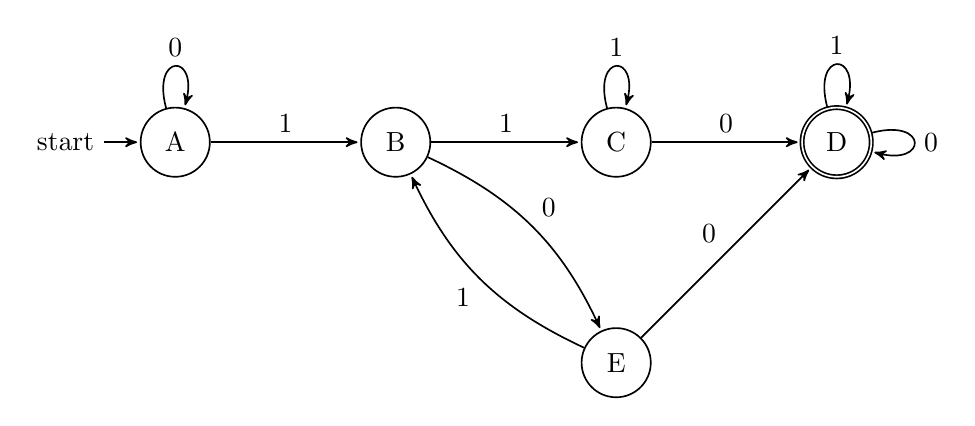
\begin{tikzpicture}[
                        ->,
                        >=stealth',
                        shorten >=1pt,
                        auto,
                        node distance=2.8cm,
                        semithick
                    ]
                    \tikzstyle{every state}=[fill=white,draw=black,text=black]

                    \node[initial,state]   (A)              {A} ;
                    \node[state]           (B) [right of=A] {B} ;
                    \node[state]           (C) [right of=B] {C} ;
                    \node[accepting,state] (D) [right of=C] {D} ;
                    \node[state]           (E) [below of=C] {E} ;

                    \path
                    (A) edge [loop above]    node {0} (A)
                    (A) edge                 node {1} (B)
                    (B) edge [bend left=20]  node {0} (E)
                    (B) edge                 node {1} (C)
                    (C) edge                 node {0} (D)
                    (C) edge [loop above]    node {1} (C)
                    (D) edge [loop right]    node {0} (D)
                    (D) edge [loop above]    node {1} (D)
                    (E) edge                 node {0} (D)
                    (E) edge [bend left=20]  node {1} (B) ;
                \end{tikzpicture}
                \label{fig:dfa:contain100110}

                \caption{A DFA to recognize strings containing at least one of
                the substrings $100$ or $110$.}
            \end{figure}
    \end{enumerate}
\end{description}

\end{document}
